% pdflatex new.tex %
\documentclass{article}

\usepackage{graphicx}
\usepackage{xcolor}
\usepackage{hyperref}
\usepackage{subcaption}

\title{Deep Learning Topic Based Sentiment Analysis and Aspect Category Detection}
\author{Berti Stefano}
\date{\today}

\begin{document}
    \thispagestyle{plain}
    % Titles %
    \begin{center}
        \Large
        \textbf{Deep Learning Topic Based Sentiment Analysis and Aspect Category Detection}

        \vspace{0.4cm}
        \large Human Language Technologies
        \\2019 / 2020

        \vspace{0.4cm}
        \textbf{Berti Stefano}

        \vspace{0.9cm}
        \textbf{Abstract}
    \end{center}
    % Abstract %
    The aim of this project is to adapt the model
    \\\centerline{\url{https://github.com/cbaziotis/datastories-semeval2017-task4}}
    to the Aspect Category Detection task and Aspect Category Polarity task of the Absita competition
    \\\centerline{\url{http://sag.art.uniroma2.it/absita}}
    I will try two different word vectors embeddings: the Italian Word2Vec embedding
    \\\centerline{\url{https://mlunicampania.gitlab.io/italian-word2vec/}}
    and the Italian BERT AlBERTo embedding
    \\\centerline{\url{http://ceur-ws.org/Vol-2481/paper57.pdf}}
    I will tune the hidden layers dimension with grid search and I will compare the results of this model with the models which won the Absita competition.

    \section{Problem description}\label{sec:s1}
        \subsection{Tasks}\label{subsec:task}
        The Absita competition is divided into 2 tasks:
        \begin{itemize}
            \item \textbf{ACD} Aspect Category Detection: given a review, understand which topics are dealt inside it from a predetermined set of topics
            \item \textbf{ACP} Aspect Category Polarity: given a review and a topic, understand if the topic is dealt in a positive, negative, neutral or mixed way
        \end{itemize}
        The second task can be seen as dependent from the first one, but I will see it as a independent task because, otherwise,
        the output errors of the first task would influence the input of the second task, and so the second task results couldn't be better than the results of the first task.
        I will use the official Absita evaluation script to test the models.
        \subsection{Dataset}\label{subsec:datset}
        The given dataset has the form
        \\\centerline{id, $t^{1}_{presence}$, $t^{1}_{+}$, $t^{1}_{-}$, \ldots , $t^{n}_{presence}$, $t^{n}_{+}$, $t^{n}_{+}$, review}
        where
        \begin{itemize}
            \item \textbf{id} is the id of the review
            \item \textbf{$t^{i}_{presence} \in \{0, 1\}$} indicate if the i-th topic in ['cleanliness', 'amenities', 'value', 'wifi', 'location', 'staff', 'other'] is dealt inside the review
            \item \textbf{$t^{i}_{+} \in \{0, 1\}$} indicate if the i-th topic is dealt in a positive/negative way, if $t^{i}_{+}$ and $t^{i}_{-}$ are both 1, then the review is mixed
            \item \textbf{review} is a string containing the raw review
        \end{itemize}
        I have two dataset files: train.csv and test.csv.
        I divided the training set into training and validation sets using the train\_test\_split function of scikit-learn with 70\%-30\% sizes, stratifying for the acp task (for the ACD task I couldn't because I can't consider combination of the topics as single classes), and with a random state of 42.
        The description of the problem also dealt with neutral reviews ($t^{i}_{presence} = 1$ and both $t^{i}_{+}$ and $t^{i}_{-} = 0$), but this combination was not present in both dataset files and so I had to exclude this sentiment in the following analysis.
        \begin{table}[h!]
            \begin{center}
                \caption{number of element for class}
                \label{tab:table1}
                \begin{tabular}{l|c|c|c|r}
                    \textbf{data} & \textbf{Training set} & \textbf{Validation set} & \textbf{Testing set}\\
                    \hline
                        number of elements & 4436 & 1901 & 2718\\
                \end{tabular}
            \end{center}
        \end{table}
        \begin{figure}
		    \centering
		    \begin{subfigure}{.5\textwidth}
  		        \centering
 		        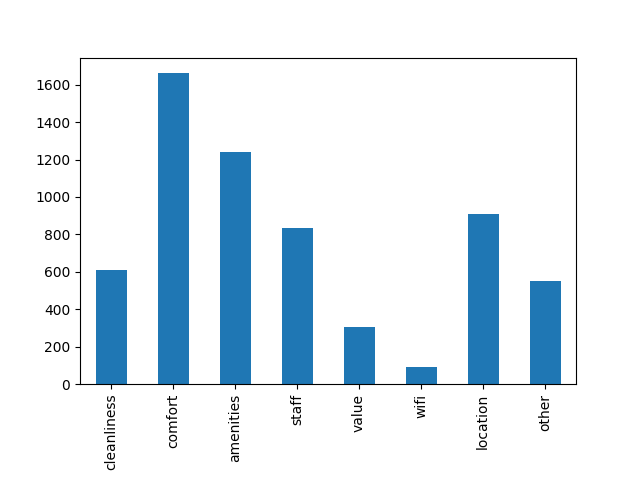
\includegraphics[width=\textwidth]{imgs/acd_y_train_historgram.png}
  		        \caption{Distribution of topics in training set for ACD task}
  		        \label{acd_y_train_historgram}
		    \end{subfigure}%
		    \begin{subfigure}{.5\textwidth}
 		        \centering
 		        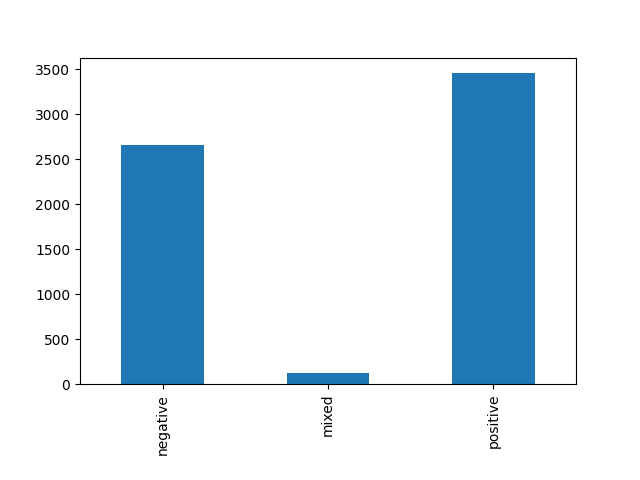
\includegraphics[width=\textwidth]{imgs/acp_y_train_historgram.png}
 		        \caption{Distribution of topics in training set for ACP task}
 		        \label{acp_y_train_historgram}
		    \end{subfigure}
		    \caption{Distribution of y in training set for both tasks}
		    \label{y_train_histograms}
	    \end{figure}
            \begin{figure}
		    \centering
		    \begin{subfigure}{.5\textwidth}
  		        \centering
 		        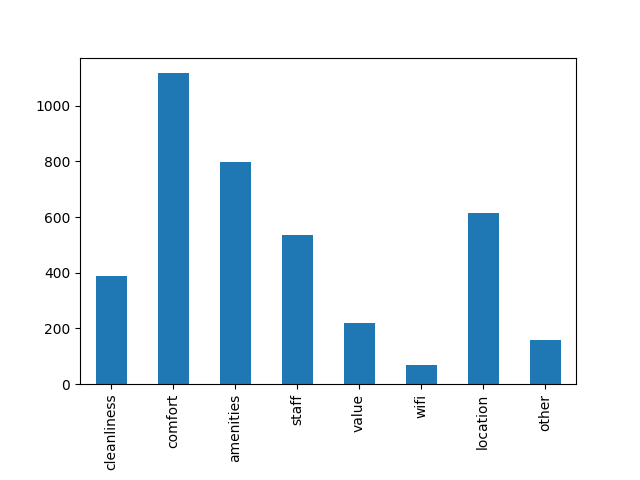
\includegraphics[width=\textwidth]{imgs/acd_y_test_historgram.png}
  		        \caption{Distribution of topics in testing set for ACD task}
  		        \label{acd_y_test_historgram}
		    \end{subfigure}%
		    \begin{subfigure}{.5\textwidth}
 		        \centering
 		        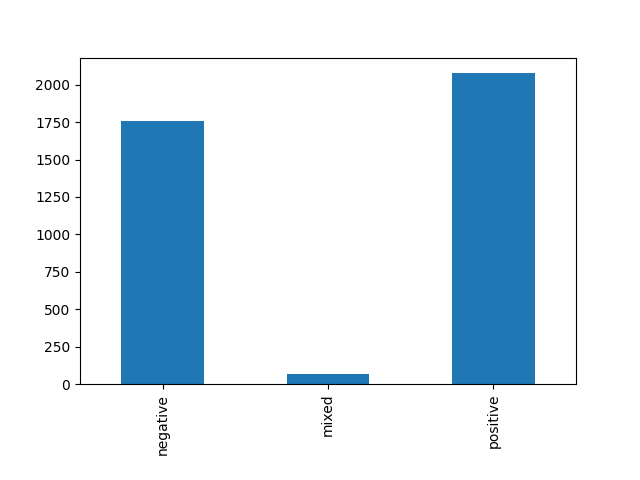
\includegraphics[width=\textwidth]{imgs/acp_y_test_historgram.png}
 		        \caption{Distribution of topics in testing set for ACP task}
 		        \label{acp_y_test_historgram}
		    \end{subfigure}
		    \caption{Distribution of y in testing set for both tasks}
		    \label{y_test_histograms}
	    \end{figure}
        \subsection{Metrics}\label{subsec:metrics}
        The metrics used in this competition in the Absita evaluation sript are micro-precision, micro-recall and f1-score.

    \section{Description of the models}\label{sec:s3}
        \begin{figure}
            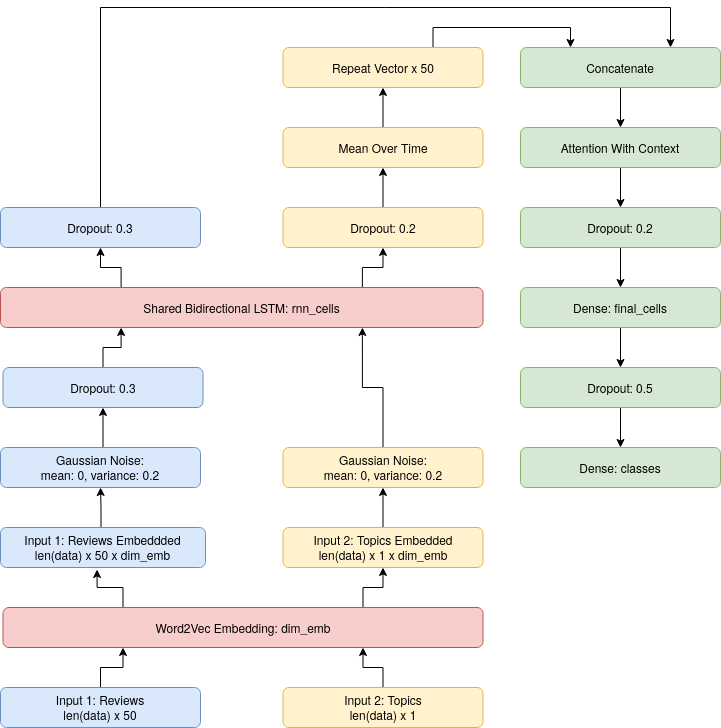
\includegraphics[width=\linewidth]{imgs/model.png}
            \caption{A general view of the model: for the alBERTo version, the reviews are already embedded, and so the input is directly feed into the BiLSTM.
            For for the w2v version, they are embedded in the Embedding Layer.
            The yellow part does not appear for the ACD task, because the task is to find those topics.
            The last dense layer has dimension 3 and softmax activation for ACP task and dimension 8 and sigmoid activation for ACD task.}
            \label{fig:model}
        \end{figure}
        \subsection{Structure of the models}\label{subsec:structure-of-the-models}
        The model chosen is the one who outperformed $Semeval2017$, which tasks were very similar to this competition.
        It is a deep-learning model with context-aware attention:
        \begin{itemize}
            \item The inputs are word indices of reviews (and topics for ACP task) to be embedded in the EmbeddingLayer for the Word2Vec version or already embedded for the AlBERTo version
            \item The reviews embeddings are fed into a shared bidirectional LSTM with rnn\_cells neurons.
                For ACP task, it does the same with the topic's embedding using the same weights in order to try to get meaningful representations
            \item For the ACP task, it concatenates each word representation with the topic representation, repeating the topic representation as many words there are in the review
            \item It uses a context-aware attention mechanism, which tries to understand which part of the reviews contribute more to the sentiment/presence towards the topic
            \item Then it is used a dense layer with final\_cells neurons
            \item Finally there is a dense layer with 8 sigmoid neuron for task ACD or 3 softmax neurons for task ACP
        \end{itemize}
        \subsection{Hyperparameters tuning}\label{subsec:hyperparameters-tuning}
            I kept the same dropout values of the original model, and I searched the best dimensions for the shared bidirectional LSTM and for the final dense layer with a grid search.
            I used {64, 128, 256} as domain, and an early stopping callback to speed up the search with delta=0.01 and patience=5 for alBERTo and patience=10 for w2v (because alBERTo learns faster than w2v), looking for maximizing the validation recall.
            I obtained the results shown in the tables (ordered by validation recall score), from which I selected the best hidden dimensions:
            \begin{itemize}
                \item w2v ACD: rnn\_cells 256, final\_cells 256
                \item w2v ACP: rnn\_cells 256, final\_cells 64
                \item alBERTo ACD: rnn\_cells 128, final\_cells 256
                \item alBERTo ACP: rnn\_cells 256, final\_cells 128
            \end{itemize}
                \begin{table}[h!]
                \begin{center}
                \caption{Grid search results for w2v ACD task}
                \label{tab:table6}
                \begin{tabular}{c|c|c|c|c}
                    \textbf{Final cells} & \textbf{BiLSTM cells} & \textbf{Accuracy} & \textbf{Epochs} & \textbf{Validation recall}\\
                    \hline
                        256 & 256 & 0.72397 & 29 & 0.77716\\
                        64  & 256 & 0.72450 & 32 & 0.76312\\
                        128 & 256 & 0.71504 & 19 & 0.76053\\
                        128 & 128 & 0.72766 & 20 & 0.75831\\
                        128 & 64  & 0.71293 & 29 & 0.75721\\
                        64  & 64  & 0.71346 & 29 & 0.75203\\
                        64  & 128 & 0.71767 & 19 & 0.74723\\
                        256 & 128 & 0.70820 & 13 & 0.74501\\
                        256 & 64  & 0.70137 & 10 & 0.73614\\
                \end{tabular}
                \end{center}
            \end{table}
            \begin{table}[h!]
                \begin{center}
                \caption{Grid search results for alBERTo ACD task}
                \label{tab:table5}
                \begin{tabular}{c|c|c|c|c}
                    \textbf{Final cells} & \textbf{BiLSTM cells} & \textbf{Accuracy} & \textbf{Epochs} & \textbf{Validation recall}\\
                    \hline
                        256 & 128 & 0.71504 & 12 & 0.77790\\
                        128 & 256 & 0.72187 & 12 & 0.77605\\
                        64  & 256 & 0.72713 & 15 & 0.77125\\
                        128 & 64  & 0.72397 & 9  & 0.75905\\
                        128 & 128 & 0.71977 & 12 & 0.74982\\
                        64  & 128 & 0.72608 & 11 & 0.74279\\
                        256 & 256 & 0.71609 & 7  & 0.73910\\
                        64  & 64  & 0.73502 & 11 & 0.73651\\
                        256 & 64  & 0.70137 & 9  & 0.73319\\
                \end{tabular}
                \end{center}
            \end{table}
            \begin{table}[h!]
                \begin{center}
                \caption{Grid search results for w2v ACP task}
                \label{tab:table7}
                \begin{tabular}{c|c|c|c|c}
                    \textbf{Final cells} & \textbf{BiLSTM cells} & \textbf{Accuracy} & \textbf{Epochs} & \textbf{Validation recall}\\
                    \hline
                        64  & 256 & 0.91246 & 29 & 0.91096\\
                        64  & 64  & 0.87767 & 22 & 0.87692\\
                        128 & 128 & 0.87580 & 13 & 0.87467\\
                        256 & 128 & 0.87392 & 14 & 0.87168\\
                        128 & 256 & 0.86944 & 13 & 0.86644\\
                        256 & 64  & 0.86756 & 17 & 0.86569\\
                        128 & 64  & 0.85597 & 9  & 0.85297\\
                        64  & 128 & 0.85597 & 6  & 0.84811\\
                        256 & 256 & 0.85036 & 3  & 0.84736\\
                \end{tabular}
                \end{center}
            \end{table}
            \begin{table}[h!]
                \begin{center}
                \caption{Grid search results for alBERTo ACP task}
                \label{tab:table3}
                \begin{tabular}{c|c|c|c|c}
                    \textbf{Final cells} & \textbf{BiLSTM cells} & \textbf{Accuracy} & \textbf{Epochs} & \textbf{Validation recall}\\
                    \hline
                        128 & 256 & 0.91545 & 6  & 0.91470\\
                        256 & 64  & 0.91770 & 10 & 0.91433\\
                        256 & 256 & 0.91358 & 6  & 0.91283\\
                        256 & 128 & 0.91470 & 12 & 0.91171\\
                        64  & 64  & 0.91470 & 6  & 0.91021\\
                        64  & 256 & 0.91246 & 10 & 0.90984\\
                        128 & 128 & 0.90311 & 8  & 0.90086\\
                        128 & 64  & 0.90161 & 5  & 0.89824\\
                        128 & 128 & 0.88178 & 4  & 0.88066\\
                \end{tabular}
                \end{center}
            \end{table}


    \section{Training best models}\label{sec:training-best-models}
        \subsection{ACP}\label{subsec:s1}
            For the ACP task I used class weights, which help dealing with imbalanced datasets by weighting more the misclassified prediction of a class
            with a limited number of example.
            In my case the class weights used were 1.26 for negative, 1.0 for positive and 8.14 for mixed.
            To generate the input for the model, I extracted tuples from the dataset with the form (sentiment, topic, review), formatting the data in such a way to repeat each review for each topic present in that review.

            \subsubsection{Word2Vec}
            Initially I made some experiments using a word embedding whose dimension was 128 (\url{http://www.italianlp.it/resources/italian-word-embeddings/}),
            but this lead to a slow and limited training, that couldn't overtake the accuracy score of 0.55.
            So I moved to a more informative embedding whose size was 300, and although the poor quality of most of the entries
            (lot of words are typo or sequence of random characters), it gave good results.
            The Italian Word2Vec embeddings (\url{https://arxiv.org/pdf/2001.09332.pdf}) are obtained from a simple 2-level neural network with one-hot vector as input.
            It has been trained with CBOW (continuous bag of words) and negative sampling, the dataset was obtained using the information extracted from a
            dump of the Italian Wikipedia (dated 2019.04.01), from the main categories of Italian Google News (WORLD, NATION, BUSINESS,
            TECHNOLOGY, ENTERTAINMENT, SPORTS, SCIENCE, HEALTH), and has a dimension of 2.4 GB .
            Embeddings are given in a txt file, but after the first loading, they are formatted as dictionary and saved in a pickle file
            to speed up following loading.
            I didn't do a lot of preprocessing of the reviews, since the embedding size is big (667564 words once removed the non-ascii ones)
            and it could cover the 85\% of the words, but looking better at the words that were indexed as $<unk>$, a lot of them were words with a capital letter.
            So by setting all chars lowercase, without losing much information because no proper name was present in the dataset, and just by removing all \textbf{l'},
            the coverage of word embeddings increased to 91.5\%.

            \begin{figure}
		    \centering
		        \begin{subfigure}{.33\textwidth}
  		            \centering
 		            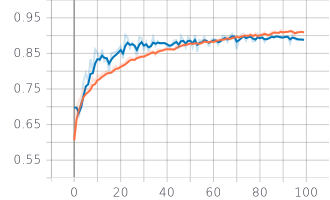
\includegraphics[width=\textwidth]{w2v_acp_epoch_accuracy.png}
  		            \caption{Distribution of topics in training set for ACD task}
  		            \label{acd_y_train_historgram1}
		        \end{subfigure}%
                \begin{subfigure}{.33\textwidth}
 		            \centering
 		            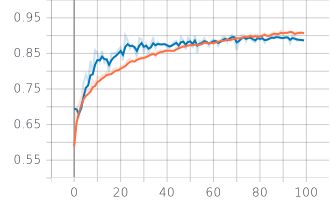
\includegraphics[width=\textwidth]{w2v_acp_epoch_recall.png}
 		            \caption{Distribution of topics in training set for ACP task}
 		            \label{acp_y_train_historgram2}
		        \end{subfigure}
                \begin{subfigure}{.33\textwidth}
 		            \centering
 		            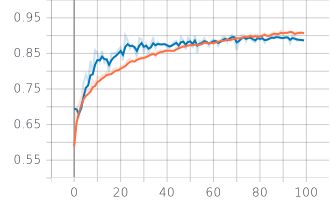
\includegraphics[width=\textwidth]{w2v_acp_epoch_recall.png}
 		            \caption{Distribution of topics in training set for ACP task}
 		            \label{acp_y_train_historgram3}
		        \end{subfigure}
		    \caption{Distribution of y in training set for both tasks}
		    \label{y_train_histograms4}
	    \end{figure}

            \color{orange} Orange is for train, \color{blue} blue is for validation.\color{black}
            \begin{figure}[!htb]
                \begin{minipage}{0.48\textwidth}
                    \centering
                    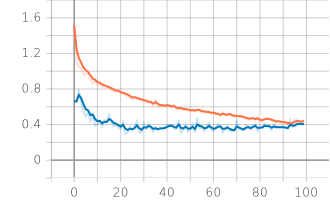
\includegraphics[width=.7\linewidth]{w2v_acp_epoch_loss.png}
                    \caption{Loss for W2V on task ACP}\label{Fig:Data1}
                \end{minipage}\hfill
                \begin{minipage}{0.48\textwidth}
                    \centering
                    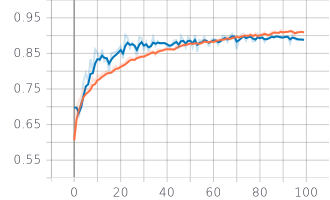
\includegraphics[width=.7\linewidth]{w2v_acp_epoch_accuracy.png}
                    \caption{Accuracy for W2V on task ACP}\label{Fig:Data2}
                \end{minipage}
                \begin{minipage}{0.48\textwidth}
                    \centering
                    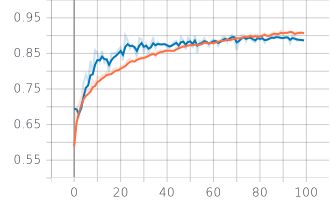
\includegraphics[width=.7\linewidth]{w2v_acp_epoch_recall.png}
                    \caption{Recall for W2V on task ACP}\label{Fig:Data3}
                \end{minipage}
            \end{figure}

            \subsubsection{AlBERTo}
            AlBERTo is the Italian BERT .
            It has the same structure of BERT, the difference is in the learning strategy: BERT is trained with "masked learning" and "next following sentence",
            while alBERTo is trained only with "masked learning".
            Because of this, alBERTo is suitable for sentiment analysis tasks, but not for more complex tasks like QA because it does not have idea of the flow of a dialogue.
            The dataset used to train alBERTo is formed by 200 million of tweets taken from TWITA, which is a big collection of tweets from 2012 since today.
            I used Huggingface Transformers to load the alBERTo model and the tokenizer, then I decided to generate an "alBERTed" version of the dataset,
            in this way I don't need to calculate the embeddings during the training because I have already computed them,
            and this result in a faster training at the cost of spending time and space once and for all to generate and save the embedded dataset.
            The alBERTo tokenizer managed to index all the words.
            The dimension of these embeddings is 768, which is much larger than the Word2Vec ones, and also this lead to better results and faster learning.
            \color{orange} Orange is for train, \color{blue} blue is for validation.\color{black}
            \begin{figure}[!htb]
                \begin{minipage}{0.48\textwidth}
                    \centering
                    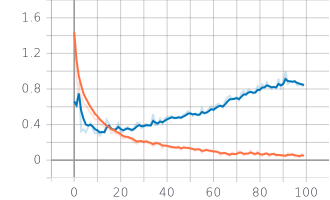
\includegraphics[width=.7\linewidth]{alberto_acp_epoch_loss.png}
                    \caption{Loss for alBERTo on task ACP}\label{Fig:Data4}
                \end{minipage}\hfill
                \begin{minipage}{0.48\textwidth}
                    \centering
                    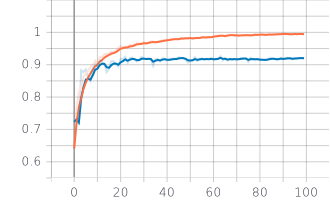
\includegraphics[width=.7\linewidth]{alberto_acp_epoch_accuracy.png}
                    \caption{Accuracy for alBERTo on task ACP}\label{Fig:Data5}
                \end{minipage}
                \begin{minipage}{0.48\textwidth}
                    \centering
                    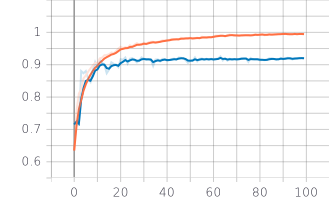
\includegraphics[width=.7\linewidth]{alberto_acp_epoch_recall.png}
                    \caption{Recall for alBERTo on task ACP}\label{Fig:Data6}
                \end{minipage}
            \end{figure}

        \subsection{ACD}\label{subsec:s2}
            Even if this model was not designed for topic-detection analysis, I wanted to test the potential of context-aware attention.
            The idea is that the context-aware attention should learn which words refers in a general way to a specific topic.
            So I modified the model in order to be able to do multi-label classification, because more topics can be dealt inside the same review.
            The approach is almost the same as for the ACP task, but I removed the part of the model which processed the topics and the output layer has dimension 8 and has a sigmoid activation.

            \subsubsection{Word2Vec}
                The input is a list of 2 numpy array: one that contains the indexed reviews and the other one that contains the indexed topics.
                The output is a numpy array with values between [0, 1] where 0 stands for "topic not dealt in this review" and 1 stands for "topic dealt in this review.
                \color{orange} Orange is for train, \color{blue} blue is for validation.\color{black}
                \begin{figure}[!htb]
                \begin{minipage}{0.48\textwidth}
                    \centering
                    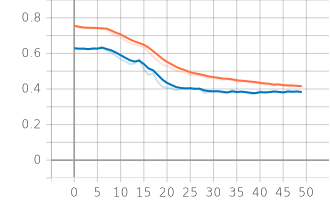
\includegraphics[width=.7\linewidth]{w2v_acd_epoch_loss.png}
                    \caption{Loss for W2V on task ACD}\label{Fig:Data7}
                \end{minipage}\hfill
                \begin{minipage}{0.48\textwidth}
                    \centering
                    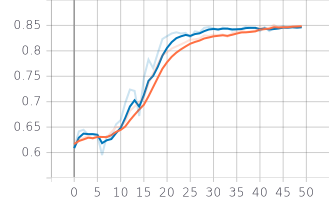
\includegraphics[width=.7\linewidth]{w2v_acd_epoch_accuracy.png}
                    \caption{Accuracy for W2V on task ACD}\label{Fig:Data8}
                \end{minipage}
                \begin{minipage}{0.48\textwidth}
                    \centering
                    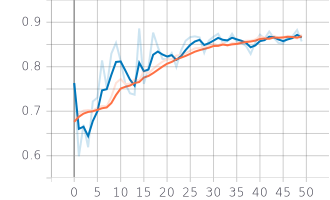
\includegraphics[width=.7\linewidth]{w2v_acd_epoch_recall.png}
                    \caption{Recall for W2V on task ACD}\label{Fig:Data9}
                \end{minipage}
            \end{figure}
            \subsubsection{AlBERTo}
                The approach is the same as before: I only need to pass the reviews to the model and for each one I will get an array of size 8 with values between [0, 1].
                \color{orange} Orange is for train, \color{blue} blue is for validation.\color{black}
                \begin{figure}[!htb]
                \begin{minipage}{0.48\textwidth}
                    \centering
                    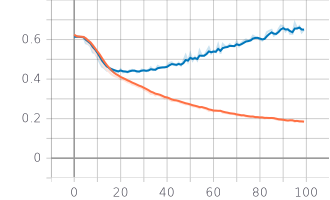
\includegraphics[width=.7\linewidth]{alberto_acd_epoch_loss.png}
                    \caption{Loss for alBERTo on task ACD}\label{Fig:Data10}
                \end{minipage}\hfill
                \begin{minipage}{0.48\textwidth}
                    \centering
                    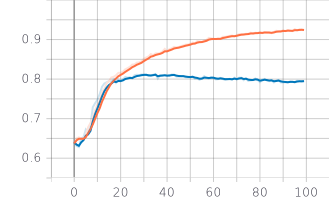
\includegraphics[width=.7\linewidth]{alberto_acd_epoch_accuracy.png}
                    \caption{Accuracy for alBERTo on task ACD}\label{Fig:Data11}
                \end{minipage}
                \begin{minipage}{0.48\textwidth}
                    \centering
                    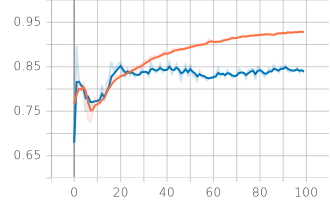
\includegraphics[width=.7\linewidth]{alberto_acd_epoch_recall.png}
                    \caption{Recall for alBERTo on task ACD}\label{Fig:Data12}
                \end{minipage}
            \end{figure}

    \section{Results}\label{sec:s5}
        As said before, I used the official evaluation\_absita script and the official gold test set for calculate the scores.
        The official evaluation script gives us also the macro measures, but the competition was based on micro measures.
                %ACD RESULTS
                \begin{table}[h!]
                    \begin{center}
                        \caption{Independent results for ACD task}
                        \label{tab:table2}
                        \begin{tabular}{l|c|c|c|r}
                            \textbf{model} & \textbf{Micro-Precision} & \textbf{Micro-Recall} & \textbf{Micro-F1-score}\\
                            \hline
                                \textbf{absita best model} & \textbf{0.8397} & \textbf{0.7837} & \textbf{0.8108}\\
                                W2V & 0.8182 & 0.7468 & 0.7808\\
                                alBERTo & 0.7993 & 0.7814 & 0.7902\\
                        \end{tabular}
                    \end{center}
                \end{table}

                \begin{table}[h!]
                    \begin{center}
                        \caption{Independent results for ACP task}
                        \label{tab:table4}
                        \begin{tabular}{l|c|c|r}
                            \textbf{model} & \textbf{Micro-Precision} & \textbf{Micro-Recall} & \textbf{Micro-F1-score}\\
                            \hline
                                absita best model & 0.8264 & 0.7161 & 0.7673\\
                                W2V & 0.9107 & 0.9006 & 0.9056\\
                                \textbf{alBERTo} & \textbf{0.9388} & \textbf{0.9248} & \textbf{0.9317}\\
                        \end{tabular}
                    \end{center}
                \end{table}
            For the ACD task, we see that both model have results very close to the winner of Absita.
            But for the ACP task, we outperform the absita best model with both embeddings by a score of more than 8 percentage points, which is a huge improvement.
            The alBERTo embedding improves the results obtained by the w2v one by more than 4 percentage points, and it also learns quite faster.

    \section{Conclusion}\label{sec:s6}
        For the ACD task, this model is not so different from the winner of Absita, but this is not surprising because this model was initially designed for the ACP task.
        model is very good at understanding the sentiment expressed toward a certain topic, and it can also understand
        if the sentiment is mixed, and if different topics have different sentiments in the same review.
        The role of the context attention is crucial in the topic based sentiment analysis, because it can understand well which words express a certain sentiment towards a certain topic.
        Also, alBERTo embeddings are much better than W2V one, in both test results and learning speed (alBERTo started overfitting after 20 epochs, w2v after 70 epochs)
        This could depend on the bigger embedding dimension (768 vs 300), the model used to obtain them
        (multiple transformers vs simple neural network) and the learning strategy (CBOW vs masked learning).

\end{document}